\documentclass[a4paper,12pt]{article}
\usepackage{tikz}
\usepackage{graphicx}
\usetikzlibrary{mindmap,trees}
\begin{document}

\title{CSP:301  Monopoly with a twist}
\author{Robin Malhotra}
\date{August 12, 2014}
\maketitle
\tableofcontents
\clearpage

\section{Introduction}

This is the design document for the CSP301 course at IIT Delhi(Fall Semester,2014).
In this course, our main aim is to create a video game version of the popular board game Monopoly. The game has to run independently on OSX, Windows and Linux with no modifications.



\section{Parts of the project}
Instead of a huge list, I find it easier to use a visual mindmap of the course. Don't worry about the tiny text, it's a vector image, so you can easily zoom in.

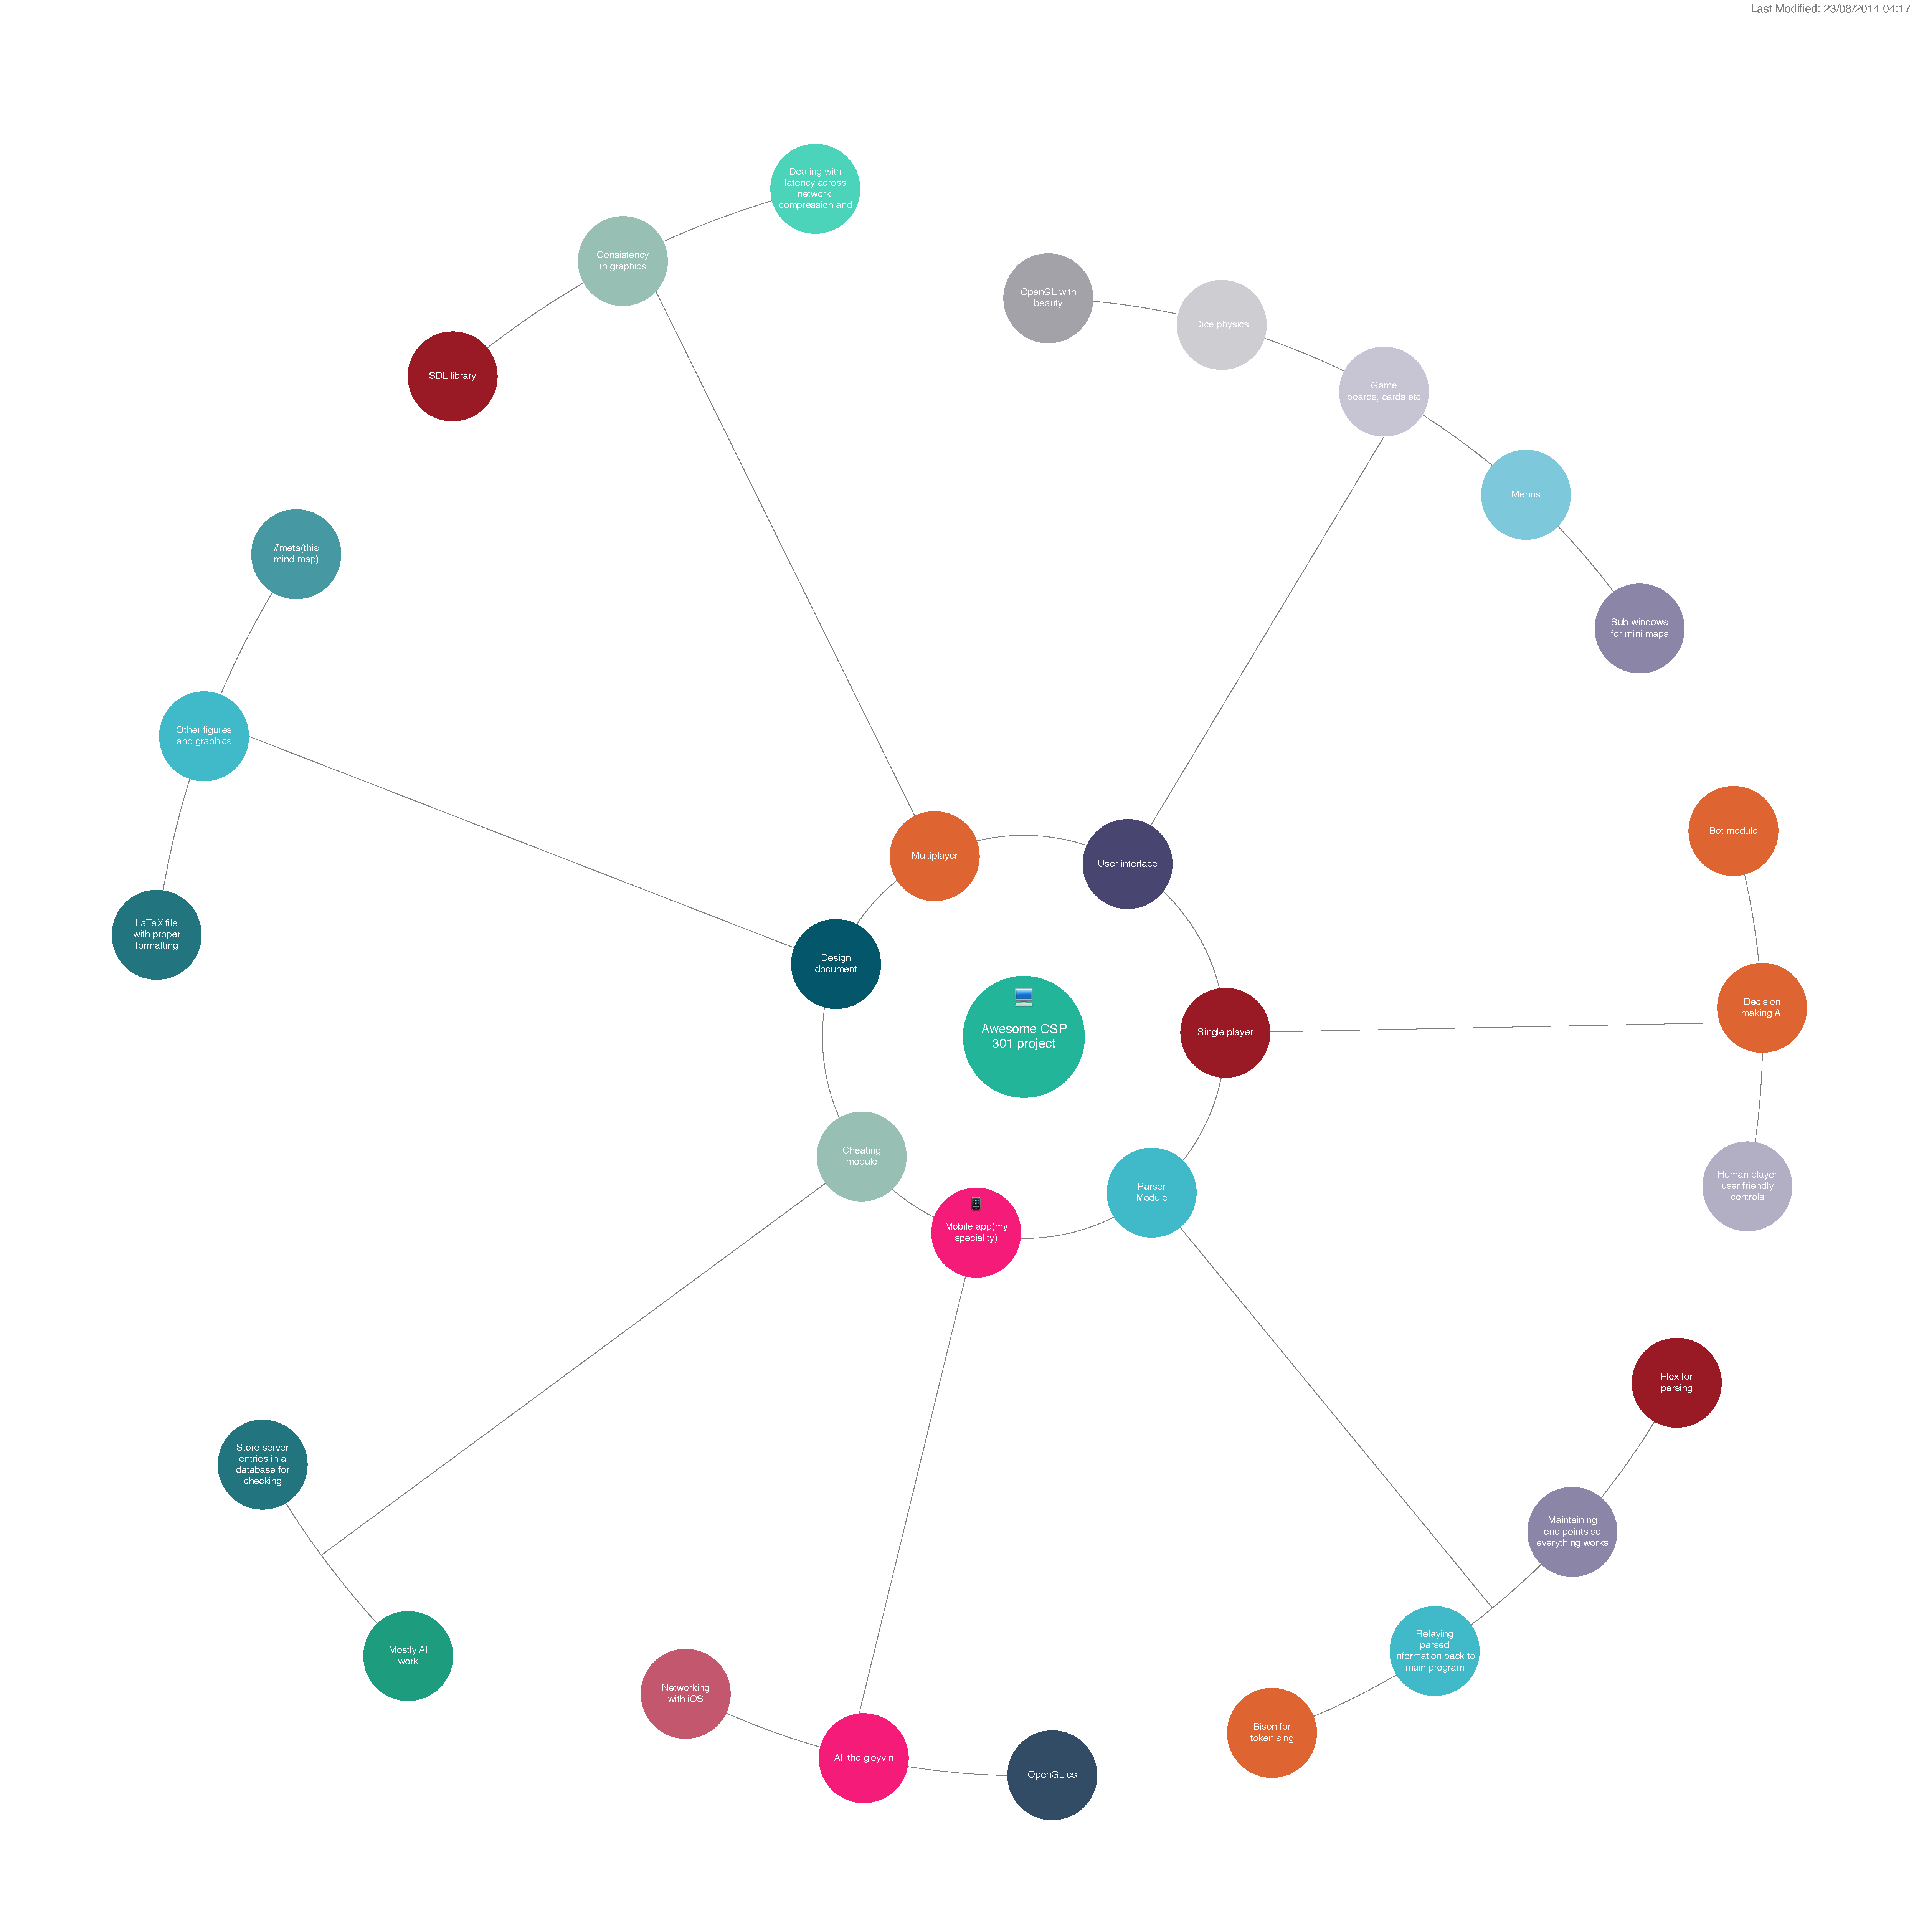
\includegraphics[width=\textwidth]{mindly.pdf}

\subsection{Parser Module}

One of the biggest requirements of the game is that the user should be able to configure the game to his/her whims and fancies by changing a config file. This will contain key-value pairs in a binary file. On game launch, it will look for the config file and change options in the game
\newline
\newline
Various customisation possibilities can include :-

\begin{itemize}
	\item{\textbf{Currency:} Various currencies with Unicode symobls. Redirect to 'credits' if no currency specified }
	\item{\textbf{Starting Money, Jail Fine and Taxes:}mostly self explanatory}
	\item{\textbf{Locations:}Range from exotic to pedestrian. Extra points for including object models with unique locations like Paris(the Eiffel Tower), New York(Statue of Liberty)}
	\item{\textbf{Railroads, electric companies etc.}}
\end{itemize}

All of this can be easily achieved with Flex and Bison. However, a faster version can be built with the config file in the JSON format. This will also be better for the mobile app(discussed later)

\subsection{User Interface}
For the user interface, I plan to use a "Age of Empires" style mini map in the game. Other nice touches can be:-
\begin{itemize}
\item{A smooth animation from the globe to the location when the user throws the dice}
\item{A deck of cards with high resolution cards}
\item{3 levels of views}

\end{document}